% https://tex.stackexchange.com/questions/428644/
\documentclass[border=5mm]{standalone}
\usepackage{tikz}
\begin{document}
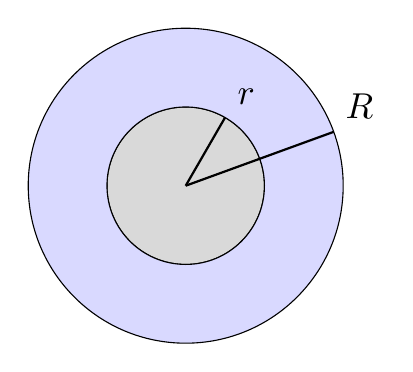
\begin{tikzpicture}[
  every node/.style={scale=1.3}
]
% inner/outer circle:
\filldraw [fill=gray!30, draw=black] (0,0) circle[radius=1];
\filldraw [fill=blue!15, draw=black, even odd rule] (0,0) circle[radius=1] circle[radius=2];
\draw [thick] (0,0) -- (60:1cm) node[anchor=225] {$r$};
\draw [thick] (0,0) -- (20:2cm) node[anchor=225] {$R$};
\end{tikzpicture}
\end{document}